\documentclass[a4paper, 12pt, titlepage]{article}

% Including needed packages
\usepackage[margin=2cm]{geometry}
\usepackage{amsmath}
\usepackage{amssymb}
\usepackage{amsthm}
\usepackage{graphicx}
\usepackage{subfig}
\usepackage{float}
\usepackage{pgf}
\usepackage{tikz}
\usepackage{dsfont}

\newcommand{\norm}[1]{\lVert#1\rVert}
\usetikzlibrary{automata,positioning}

\title
{{\em Machine learning 2}\\
Exercise sheet 10}
\author{FLEISCHMANN Kay, Matrnr: 352247\\
	ROHRMANN Till, Matrnr: 343756}
\date{\today}

\begin{document}

\maketitle
\section*{Hidden Markov Model}

Let $A_{i,j}$ the transition matrix between hidden states $x_i$ and $x_j$. $B_{i,j}$ is the the probability, beeing in state $x_i$ to observe $y_j$.
The following matrices $A$ and $B$ describe two hidden states and two possible observations.

\[
A= 
 \begin{pmatrix}
  0.1 & 0.9 \\
  0.5 & 0.5
 \end{pmatrix}
\]

\[
B=
 \begin{pmatrix}
  0.2 & 0.8 \\
  0.4 & 0.6
 \end{pmatrix}
\]

The Hidden-Markov-chain for $A$ and $B$ looks like the following4

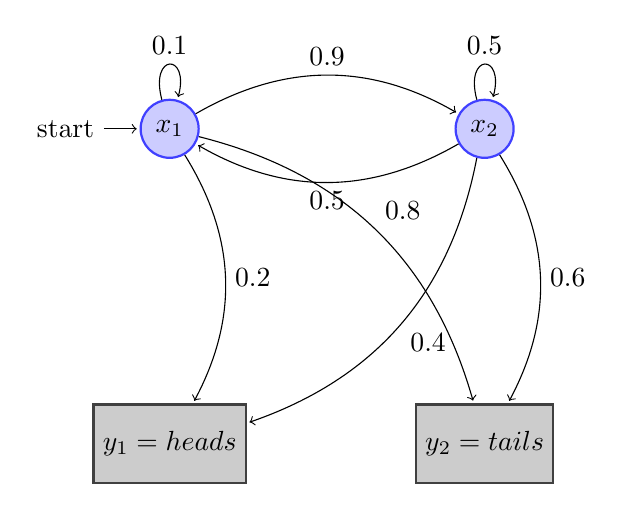
\begin{tikzpicture}[shorten >=1pt,node distance=2cm,on grid,auto] 
  \tikzstyle{state}=[circle,thick,draw=blue!75,fill=blue!20,minimum size=6mm]
  \tikzstyle{observation}=[rectangle,thick,draw=black!75,
  			  fill=black!20,minimum size=10mm]
  			  
  \node[state,initial] (x1)   {$x_1$};
  \node[state] (x2) [right=4cm of x1] {$x_2$};
  \node[observation] (y1) [below=4cm of x1] {$y_1=heads$};
  \node[observation] (y2) [right=4cm of y1] {$y_2=tails$};

  \path[->] (x1) edge [bend left] node {0.9} (x2);
  \path[->] (x2) edge [bend left] node {0.5} (x1);
  \path[->] (x1) edge [loop above] node {0.1} (x1);
  \path[->] (x2) edge [loop above] node {0.5} (x2);

  \path[->] (x1) edge [bend left] node {0.2} (y1);
  \path[->] (x1) edge [bend left] node {0.8} (y2);

  \path[->] (x2) edge [bend left] node {0.4} (y1);
  \path[->] (x2) edge [bend left] node {0.6} (y2);
\end{tikzpicture}

\subsection*{(a) Implementation of Viterbi algorithm} 
\subsection*{(b) Experiment} 


\end{document}